\documentclass{standalone}

\usepackage{tikz}
\usepackage{circuitikz}

\tikzset{block/.style = {draw, fill=white, very thick, rectangle, minimum height=1cm, minimum width=2cm},
         lblock/.style={draw,fill=white,very thick, rectangle, minimum height=3cm, minimum width=1cm},
         sum/.style= {draw, fill=white, very thick, circle, node distance=0.5cm}}

         
\begin{document}
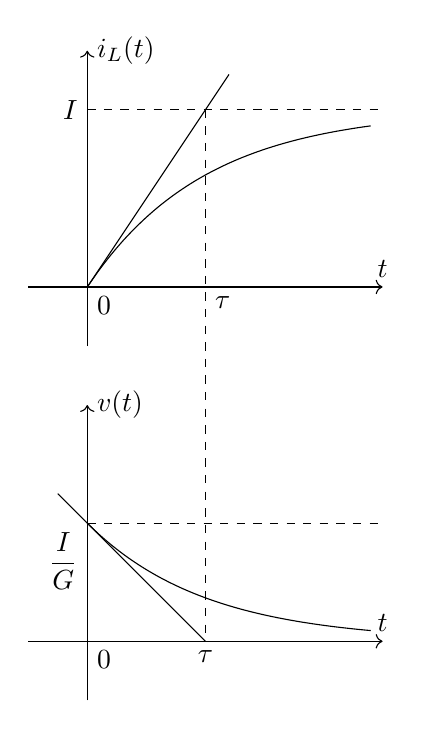
\begin{tikzpicture}[scale=1.5]
    \draw[->](0,-0.5)--(0,2)node[right]{$i_L(t)$};
    \draw[->](-0.5,0)--(2.5,0)node[above]{$t$};
    \draw[dashed](0,1.5)node[left]{$I$}--(2.5,1.5);
    \draw[-]plot[smooth, domain=0:2.4](\x,{1.5*(1-e^(-\x))});
    \draw[-](0,0)node[below right]{$0$}--(1.2,1.8);

    \draw[->](0,-3.5)--(0,-1)node[right]{$v(t)$};
    \draw[->](-0.5,-3)--(2.5,-3)node[above]{$t$};
    \draw[dashed](0,-2)node[below left]{$\displaystyle\frac{I}{G}$}--(2.5,-2);
    \draw[-]plot[smooth, domain=0:2.4](\x,{e^(-\x)-3});
    \draw[-](1,-3)--(-0.25,-1.75);
    \node[below right]at(0,-3){$0$};
    \draw[dashed](1,1.5)--(1,0)node[below right]{$\tau$}--(1,-3)node[below]{$\tau$};
\end{tikzpicture}
\end{document}